
\subsubsection{Quality test-2: Rotation test}
The test-2 (presented in the Algorithm \ref{alg:rotationtest} of Section \ref{sec:algorithm}) 
shows the correlations between two square analysis regions 
($B_0$ and $B_i$),
of $WSIZE$ pixels of side; so that $B_i$ is a rotated version, an angle $\alpha_i=0.5 i$, 
of analysis region $B_0$, $\forall~i\in Z^+~|~0  \leq  i \leq 23$. 
The purpose of this test is to know the lost of correlation when the body under study
suffers a distortion  that causes a rotation of the analysis region $B_0$.
Thus, the Figs. \ref{fig:choosingr16}, \ref{fig:choosingr32} and \ref{fig:choosingr64}
show the correlation values for two analysis regions rotated until an angle of $\alpha_{max}=11.5^\circ$,
in each figure is shown the behavior to the 3 types of patterns. Being that the Fig. \ref{fig:choosingr16}
use a $WSIZE=16$, the Fig. \ref{fig:choosingr32} a $WSIZE=32$ and the last a $WSIZE=64$.
\begin{figure}[H]
  \centering
  \begin{subfigure}[b]{0.45\textwidth}
    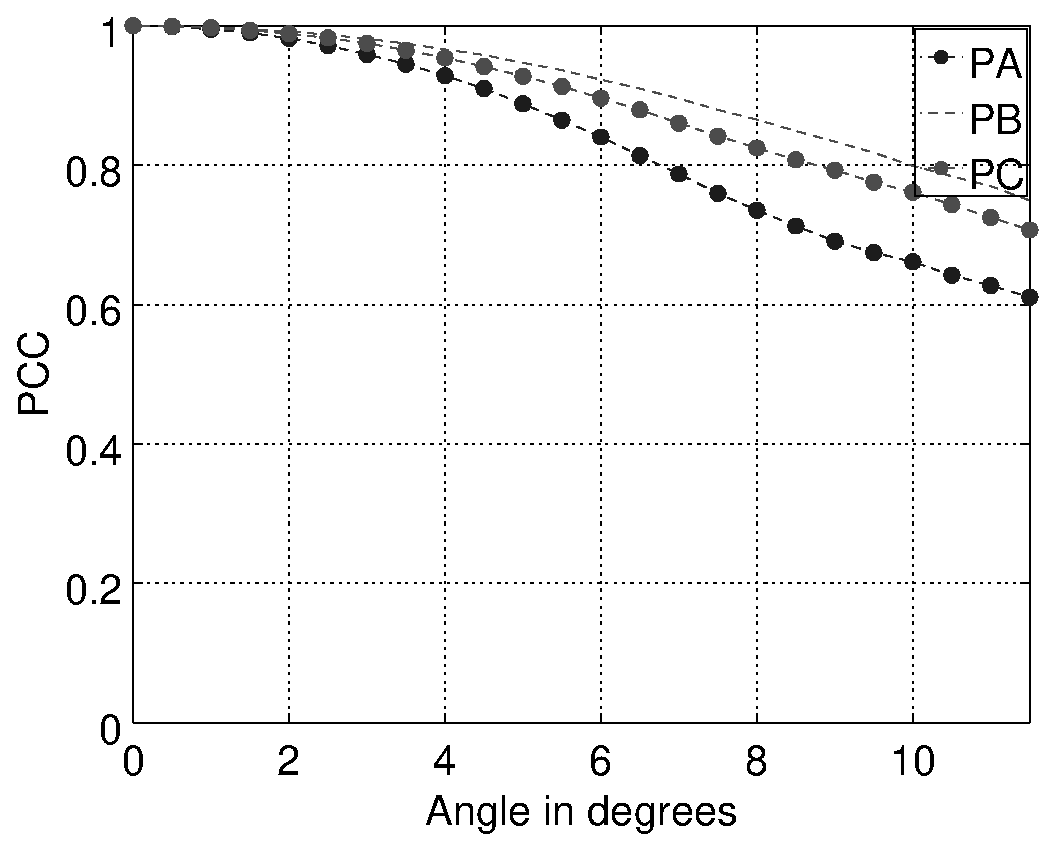
\includegraphics[width=\textwidth]{image_rot_plot-16.eps}
    \vspace{2pt}
    \caption{Rotation test to $WSIZE=16$.}
    \label{fig:choosingr16}
  \end{subfigure}
  \begin{subfigure}[b]{0.45\textwidth}
    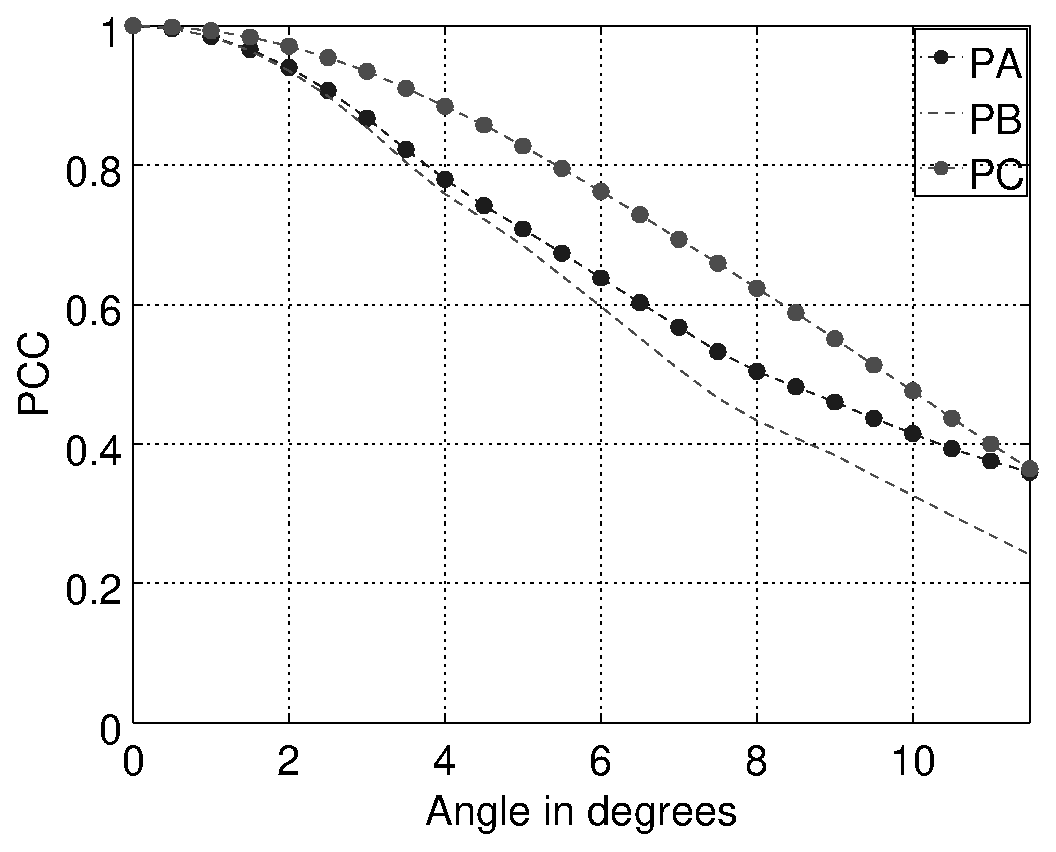
\includegraphics[width=\textwidth]{image_rot_plot-32.eps}
    \vspace{2pt}
    \caption{Rotation test to $WSIZE=32$.}
    \label{fig:choosingr32}
  \end{subfigure}
  \begin{subfigure}[b]{0.45\textwidth}
    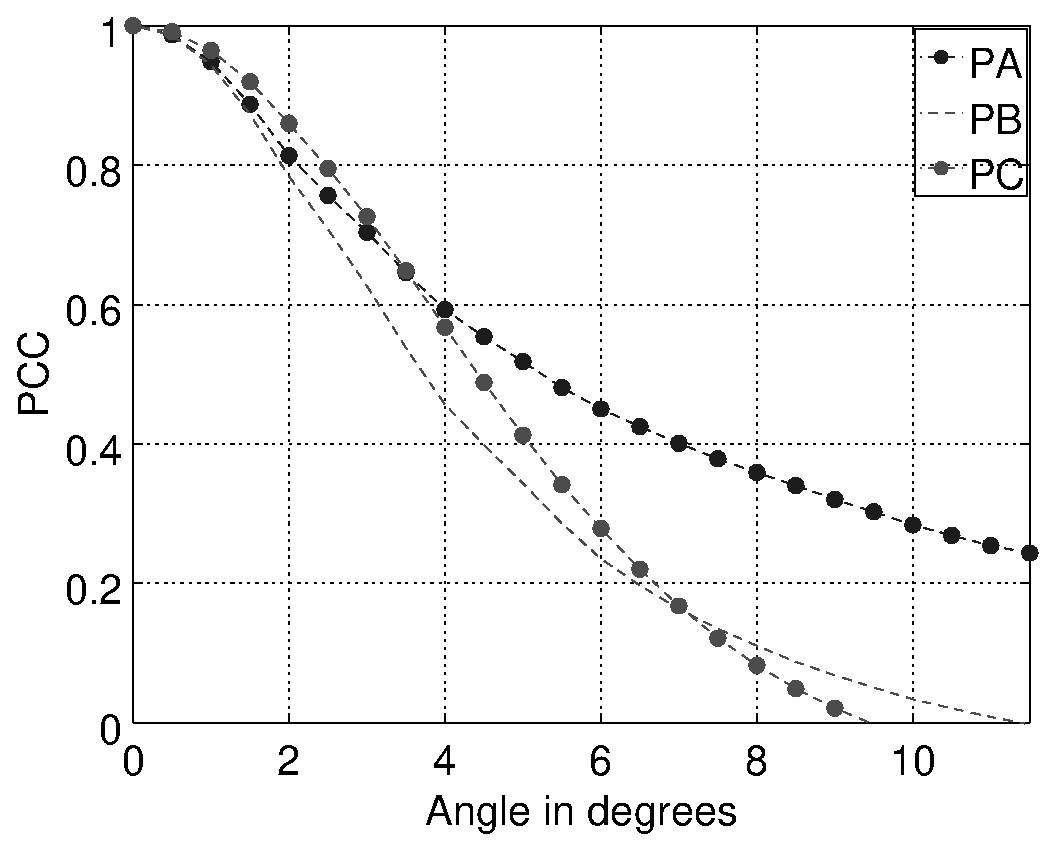
\includegraphics[width=\textwidth]{image_rot_plot-64.eps}
    \vspace{2pt}
    \caption{Rotation test to $WSIZE=64$.}
    \label{fig:choosingr64}
  \end{subfigure}
  \caption{Rotation test to different values of analysis region side $WSIZE$.}
  \label{fig:RotationAll}
\end{figure}

The Fig. \ref{fig:choosingr16} shows a low correlation loss by the 
rotation of a region $B_0$ in all patterns; being that the patterns $PB$ and $PC$ have
the best response to the rotation, holding a $PCC>0.7$ to rotation angles minors that $11.5^\circ$.
This meaning that using a threshold value of $0.7$, the $PIV$ technique in the patterns $PB$ and $PC$
can identify the region $B_0$, even if it has been rotated, up to an angle of $11.5^\circ$;
and the patterns $PA$ to the same threshold only supports a maximum rotation of an angle of $8.25^\circ$.
In a similar way, using a threshold value of $0.7$, in the Fig. \ref{fig:choosingr32},
the patterns $PA$ and $PB$ only support a maximum rotation of an angle of $5.0^\circ$, and
the pattern $PC$ an angle of $7.0^\circ$.
Finally, using the same threshold, in the Fig. \ref{fig:choosingr64},
the patterns $PA$, $PB$ and $PC$ only support a maximum rotation of an angle of $3.0^\circ$, approximately.

In general is evident that, when the value $WSIZE$ grow up, the maximum angle that support the
$PIV$ technique to recognize a rotated region, decreases.


